\section{A weak Potts field as a tilt}\label{sec:frontier-modes}

In this section the start is uniform again. For $h=(h_1,\ldots,h_d)\in\mathbb R^d$
define the \emph{tilted occupation law}
\begin{equation}\label{eq:weakfield-law}
 \widetilde P_{N,h}(n)=
 \frac{e^{h\cdot n/N}P_N(n)}
 {\sum_{m_1+\cdots+m_d=N}e^{h\cdot m/N}P_N(m)}.
\end{equation}
We use the window coordinate $T=L-\frac12\log L+t$. The normalizing sum cancels
whenever we compare 2 bins. When we speak of a modal phase we mean the support
of the global modes, which need not be the face with most of the mass
(Remark~\ref{rem:mass-mode}).

\begin{proposition}[the field is a tilt]\label{prop:field-tilt}
Let $\Lambda_N(h)=\log\E\exp\langle h,K_N/N\rangle$.
\begin{enumerate}[(1)]
\item $\widetilde P_{N,h}(n)=\exp\bigl(\langle h,n/N\rangle-\Lambda_N(h)\bigr)P_N(n)$.
So $\widetilde P_{N,h}$ is the exponential tilt of the law of the occupation
rate $K_N/N$ by the linear function $\langle h,\cdot\rangle$.
\item It is also the law of the counts when the law of the path is tilted by
$\exp(\sum_{s=1}^Nh_{X_s}/N)$. This is the Potts chain with free boundaries,
coupling $p/r$ per equal neighbor pair and field $h/N$ at each site.
\item If $T\to\infty$, then $\Lambda_N(h)\to\bar h=\frac1d\sum_ih_i$.
\end{enumerate}
\end{proposition}

\begin{proof}
Part (1) is~\eqref{eq:weakfield-law} with its denominator written as
$e^{\Lambda_N(h)}$. For (2), a word $x_1\cdots x_N$ has probability
$\frac1dr^{N-1}(p/r)^{\sum_{s<N}\delta(x_s,x_{s+1})}$, and
$\sum_sh_{x_s}=\langle h,n\rangle$ depends on the word only through its counts
$n$. So tilting the words and then counting gives (1). For (3), the chain is
stationary with transition matrix $\sigma I+(1-\sigma)\frac1dJ$, whose $m$-th
power is $\sigma^mI+(1-\sigma^m)\frac1dJ$. So $\E K_{N,a}=N/d$, and the
indicators of state $a$ at times $s$ and $s+m$ have covariance
$\sigma^m(\frac1d-\frac1{d^2})$. Summing over the 2 times gives, for $p<1$,
\[
 \Var K_{N,a}=\Bigl(\frac1d-\frac1{d^2}\Bigr)
 \Bigl(N\,\frac{1+\sigma}{1-\sigma}-\frac{2\sigma(1-\sigma^N)}{(1-\sigma)^2}\Bigr).
\]
Since $1-\sigma=dr$, for $1/d\le p<1$ the second term in the bracket is not
positive and $\Var(K_{N,a}/N)\le2/(d^2T)$. For $p<1/d$ the bracket is at most
$N+4$ while $T\le N$. So $\Var(K_{N,a}/N)=O(1/T)$, and $K_N/N$ tends to the
uniform vector in probability. Since $\exp\langle h,K_N/N\rangle$ is bounded,
bounded convergence gives the limit.
\end{proof}

Note the scale. By (1), $|\log\widetilde P_{N,h}(n)-\log P_N(n)|\le2\max_i|h_i|$
for every $n$. In the window this is of order 1, the same order as the
constants $a_k$ that break the tie. At first order, with $T=\tau L$, it is
invisible, so a field of total size $o(\log N)$ does not change the first-order
face selection of Paper~C~\cite{paperC}. The Potts chain in a field is exactly
solvable in the thermodynamic limit~\cite{kassanogly2003}, but here $N$ is
finite and the field has size $h_i/N$. For a support $S$ with $|S|\ge2$ put
$\bar h_S=\frac1{|S|}\sum_{i\in S}h_i$.

\begin{theorem}[weak-field modal phase diagram]\label{thm:weakfield-phases}
Put $T=L-\frac12\log L+t$ and define the face scores
\[
 \ell_S(t,h)=
 \begin{cases}
 h_i,& S=\{i\},\\
 (|S|-1)(t-a_{|S|})+\bar h_S,& |S|\ge2.
 \end{cases}
\]
The largest bin weight, taken relative to the untilted vertex before
normalizing~\eqref{eq:weakfield-law}, satisfies
\begin{equation}\label{eq:weakfield-maximum}
 \log\max_n\left\{e^{h\cdot n/N}\frac{P_N(n)}{V_N}\right\}
 \longrightarrow \max_{\varnothing\ne S\subseteq\{1,\ldots,d\}}
 \ell_S(t,h).
\end{equation}
For fixed $(t,h)$ and all large $N$, every global mode has a support that
maximizes the limiting score. If the maximizing support is unique, all global
modes have exactly that support. On a selected support $S$ with $|S|\ge2$,
their locations satisfy
\[
 \max_{i\in S}\left|\frac{n_i}{N}-\frac1{|S|}\right|=o((\log N)^{-1/2}).
\]
This does not identify the maximizing vectors exactly, and equal limiting
scores do not imply that both supports hold modes at finite $N$.

If the fields are sorted as $h_1\ge\cdots\ge h_d$, the maximum of the scores is
the upper envelope of the $d$ lines
\begin{equation}\label{eq:weakfield-lines}
 \ell_1(t)=h_1,\qquad
 \ell_k(t)=(k-1)(t-a_k)+\frac1k\sum_{i=1}^k h_i,
 \quad 2\le k\le d.
\end{equation}
Away from ties, the winning support size is nondecreasing in $t$. If the fields
are strictly ordered, the winning supports are the nested sets
$\{1,\ldots,k\}$. Every support size $k\in\{2,\ldots,d-1\}$ is the unique
winning size on an open interval of $t$ for suitable fixed fields. So
proper-face phases persist under a field of order $1/N$ per step.
\end{theorem}

On a support $S$ the tilt multiplies the Gaussian profile of
the ratio to a vertex (Lemma~\ref{lem:confinement}) by $e^{h\cdot n/N}$, which
is $e^{\bar h_S+o(1)}$ near the center of the face. So the best bin on $S$
scores $\ell_S(t,h)$, and taking the $k$ largest fields gives the lines. The
proof is in Appendix~\ref{app:start-field}.

\begin{remark}[how many bins beat a vertex]\label{rem:frontier-superlevel}
The same profile counts the bins that beat a vertex. Put $h_*=\max_ih_i$ and,
for a support $S$ with $|S|=k\ge2$, $B_S(t,h)=\ell_S(t,h)-h_*$. Let $M_{N,S}(t,h)$
be the number of bins with support exactly $S$ whose tilted probability is
strictly greater than that of every vertex. Then, uniformly for $(t,h)$ in
compact sets,
\[
 \frac{L^{(k-1)/2}}{N^{k-1}}M_{N,S}(t,h)
 \longrightarrow
 \frac{|\mathbb B_{k-1}|}{\sqrt k}
 \left(\frac{4\,[B_S(t,h)]_+}{k^2}\right)^{(k-1)/2},
\]
where $|\mathbb B_{k-1}|$ is the volume of the unit ball in $\mathbb R^{k-1}$
and $[x]_+=\max(x,0)$ (proof omitted). In the coordinates
$y=\sqrt L\,(n/N-\frac1k\mathbf1)$ these bins fill a ball of squared radius
$4B_S/k^2$, and $\sqrt k\,(\sqrt L/N)^{k-1}$ is the covolume of the lattice of
the points $y$. For $k=2$ the constant is $\sqrt{2[t-a_2]_+}$, which agrees with
the binary window of Paper~A once the different centering is taken into
account. The profile and the lattice volumes are checked numerically, and the
covolume $\sqrt k$ is checked in Lean.
\end{remark}

So the field shifts each face line by the field averaged over the face. On
$K_d$ the quasi-ergodic law of a face, the product of its left and right Perron
vectors in Paper~C, is uniform on the face, and $\bar h_S$ is the average of $h$
under it. For a general generator $Q$ we have
$P_N\operatorname{diag}(e^{h/N})=I+\frac TN(Q+\operatorname{diag}(h)/T)+O(T/N^2)$,
so the field acts as a potential $h/T$ added to $Q$. First-order perturbation of
the Perron root then lowers $T\lambda_F$ by $\langle h,\alpha^*_F\rangle+O(1/T)$,
where $\alpha^*_F$ is the quasi-ergodic law. So we expect each face line to gain
$\langle h,\alpha^*_F\rangle$ in general, but we have not written this out.

\begin{example}[a persistent triangular edge phase]\label{ex:weakfield-triangle}
For $d=3$ and $h=(0,0,-H)$ the 3 competing scores are $0$, $t-a_2$ and
$2(t-a_3)-H/3$. If $H>6(a_2-a_3)$, the edge $\{1,2\}$ wins strictly for
\[
 a_2<t<H/3+2a_3-a_2,
\]
and for every fixed $t$ in this interval all global modes of the tilted law lie
on that edge for large $N$. Without a field no proper face holds a mode in the
window (Corollary~\ref{cor:simplex-modes}).
\end{example}

\begin{remark}[start versus field]\label{rem:start-vs-field}
Compare a start $\mu$ with full support and no field
(Remark~\ref{rem:start-modes}) with the uniform start and the field
$h_i=\log(d\mu_i)$ (Theorem~\ref{thm:weakfield-phases}). We add $\log d$ to the
start lines, which does not change the modes. Then a vertex $i$ scores
$\log(d\mu_i)$ in both. A support $S$ with $k\ge2$ states scores $(k-1)(t-a_k)$
plus the logarithm of the arithmetic mean of $d\mu$ on $S$ under the start, and
plus the logarithm of the geometric mean under the field. The arithmetic mean is
at least the geometric mean, with equality only when $\mu$ is constant on $S$.
So a start favors mixed faces more than the field with the same vertex scores.
For example, in Remark~\ref{ex:K3-start} state 3 has start weight 0, which as
a field would mean $H=\infty$, and yet the edge window has width only $0.026$.
We have not written out the lines for a start and a field together.
\end{remark}

\begin{corollary}[one field realizes the full face hierarchy]
\label{cor:weakfield-full-hierarchy}
Fix $d\ge2$ and $H>3/4$, and let $h_i=-H(i-1)^2$ for $1\le i\le d$. In
particular $h_i=-(i-1)^2$ works in every fixed dimension. Put
\[
 c_k=(k+\tfrac12)\log k-\frac{k-1}{2}\log(4\pi),\qquad
 t_k=c_k-c_{k+1}+\frac{H(4k-1)}6\quad(1\le k<d),
\]
and $t_0=-\infty$, $t_d=+\infty$. Then $t_1<\cdots<t_{d-1}$, and for every
$k\in\{1,\ldots,d\}$ the support $\{1,\ldots,k\}$ is the unique winning support
on the nonempty interval $t_{k-1}<t<t_k$. So for each fixed $t$ in this
interval and all large $N$, every global mode of the tilted law has exactly
those $k$ positive coordinates.
\end{corollary}

Here $c_1=0$ and $c_k=\log D_k$ for $k\ge2$. Figure~\ref{fig:phases} shows the
lines for $d=5$, and the proof is in Appendix~\ref{app:start-field}.

\begin{figure}[t]
\centering
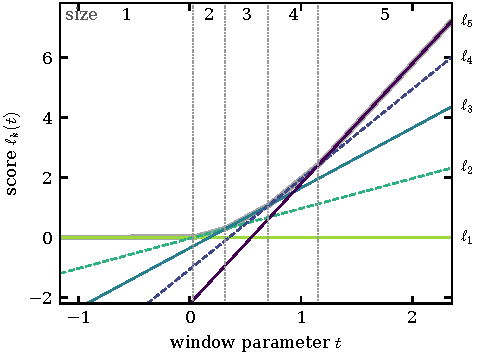
\includegraphics{figures/phases}
\caption{The lines~\eqref{eq:weakfield-lines} for $d=5$ and $h_i=-(i-1)^2$. The
grey band is their upper envelope. The dotted lines are $t_1<\cdots<t_4$, and
the number at the top of each interval is the size $k$ of the winning support
$\{1,\ldots,k\}$.}
\label{fig:phases}
\end{figure}

\begin{remark}[sticky priors]\label{rem:sticky}
Our chain is Paper~C's sticky chain with the uniform kernel. Paper~C normalizes
that chain by $Q=(J-dI)/(d-1)$, so its $T$ and $\tau$ are $d-1$ times ours, and
the tie at our $T=L$ sits at its $\tau=d-1$. The uniform kernel meets Paper~C's
direct-jump criterion with equality for every face. For $d\ge3$ and a symmetric
kernel with all off-diagonal rates positive, Paper~C shows that only the
uniform kernel meets this criterion, so only it ties on every face at first
order. The tie then resolves as a direct jump
(Corollary~\ref{cor:simplex-modes}), while a field
(Corollary~\ref{cor:weakfield-full-hierarchy}) or a start that is not uniform
(Remark~\ref{ex:K3-start}) puts intermediate faces inside the window, of width
$O(1/N)$ in $p$. If the path is observed through a likelihood with
log-likelihood $\langle h,n\rangle/N$, then $\widetilde P_{N,h}$ is the posterior
law of the counts. Kernels that are not uniform act at first order in Paper~C, on
the scale $L$ in $T$, and the field and the start only at order 1, so they are
not interchangeable.
\end{remark}

\begin{remark}[mass versus mode]\label{rem:mass-mode}
From each state of a face $F$ with $k$ states the chain stays in $F$ with
probability $1-(d-k)r$, so $\Prob(\supp K_N\subseteq F)=\mu(F)(1-(d-k)r)^{N-1}$.
So the bins with full support have mass at least
$1-\sum_{|F|=d-1}\mu(F)(1-r)^{N-1}=1-O(e^{-T})$, while for the uniform start,
$t<a_d$ and large $N$ the modes are single states
(Corollary~\ref{cor:simplex-modes}).
\end{remark}
